\chapter{Design}

\subsection{Architecture}

\begin{center}
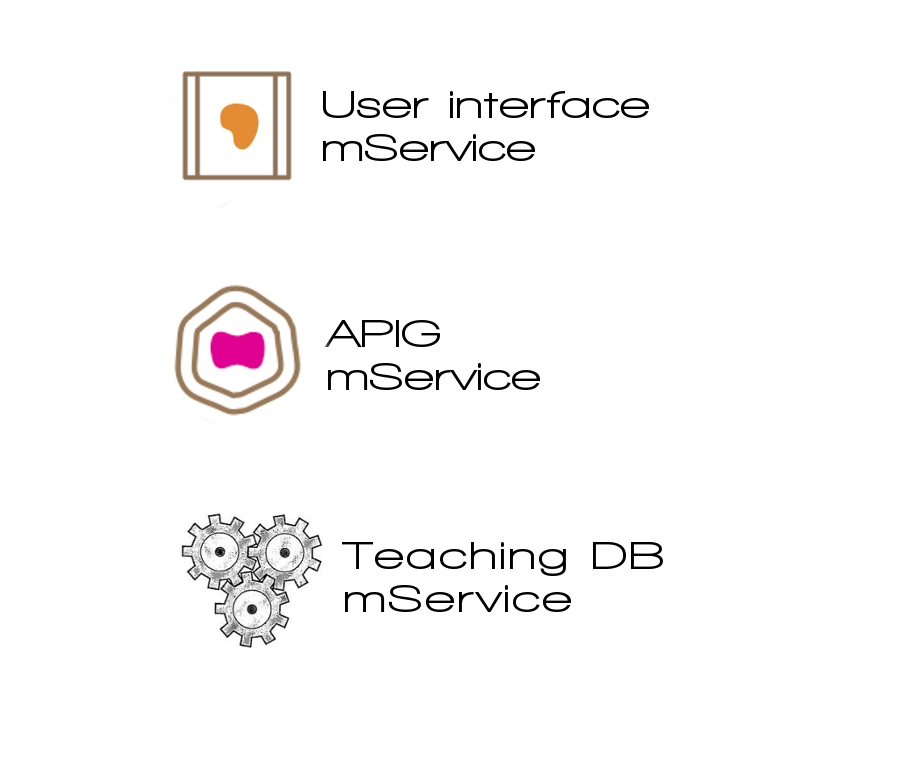
\includegraphics[scale=0.3]{img/graphics/initial_microservices_distribution.png}
\end{center}

\begin{center}
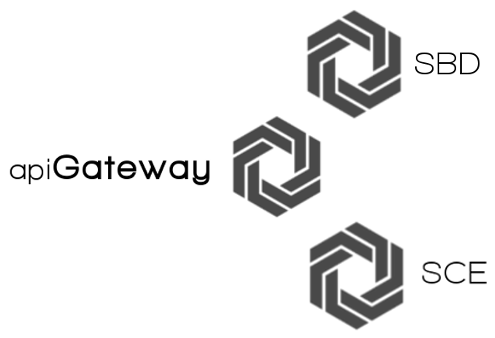
\includegraphics[scale=0.3]{img/graphics/backend.png}
\end{center}




This is the complete snap of the system in their final distribution of the
fuctionality between the services.

\begin{center}
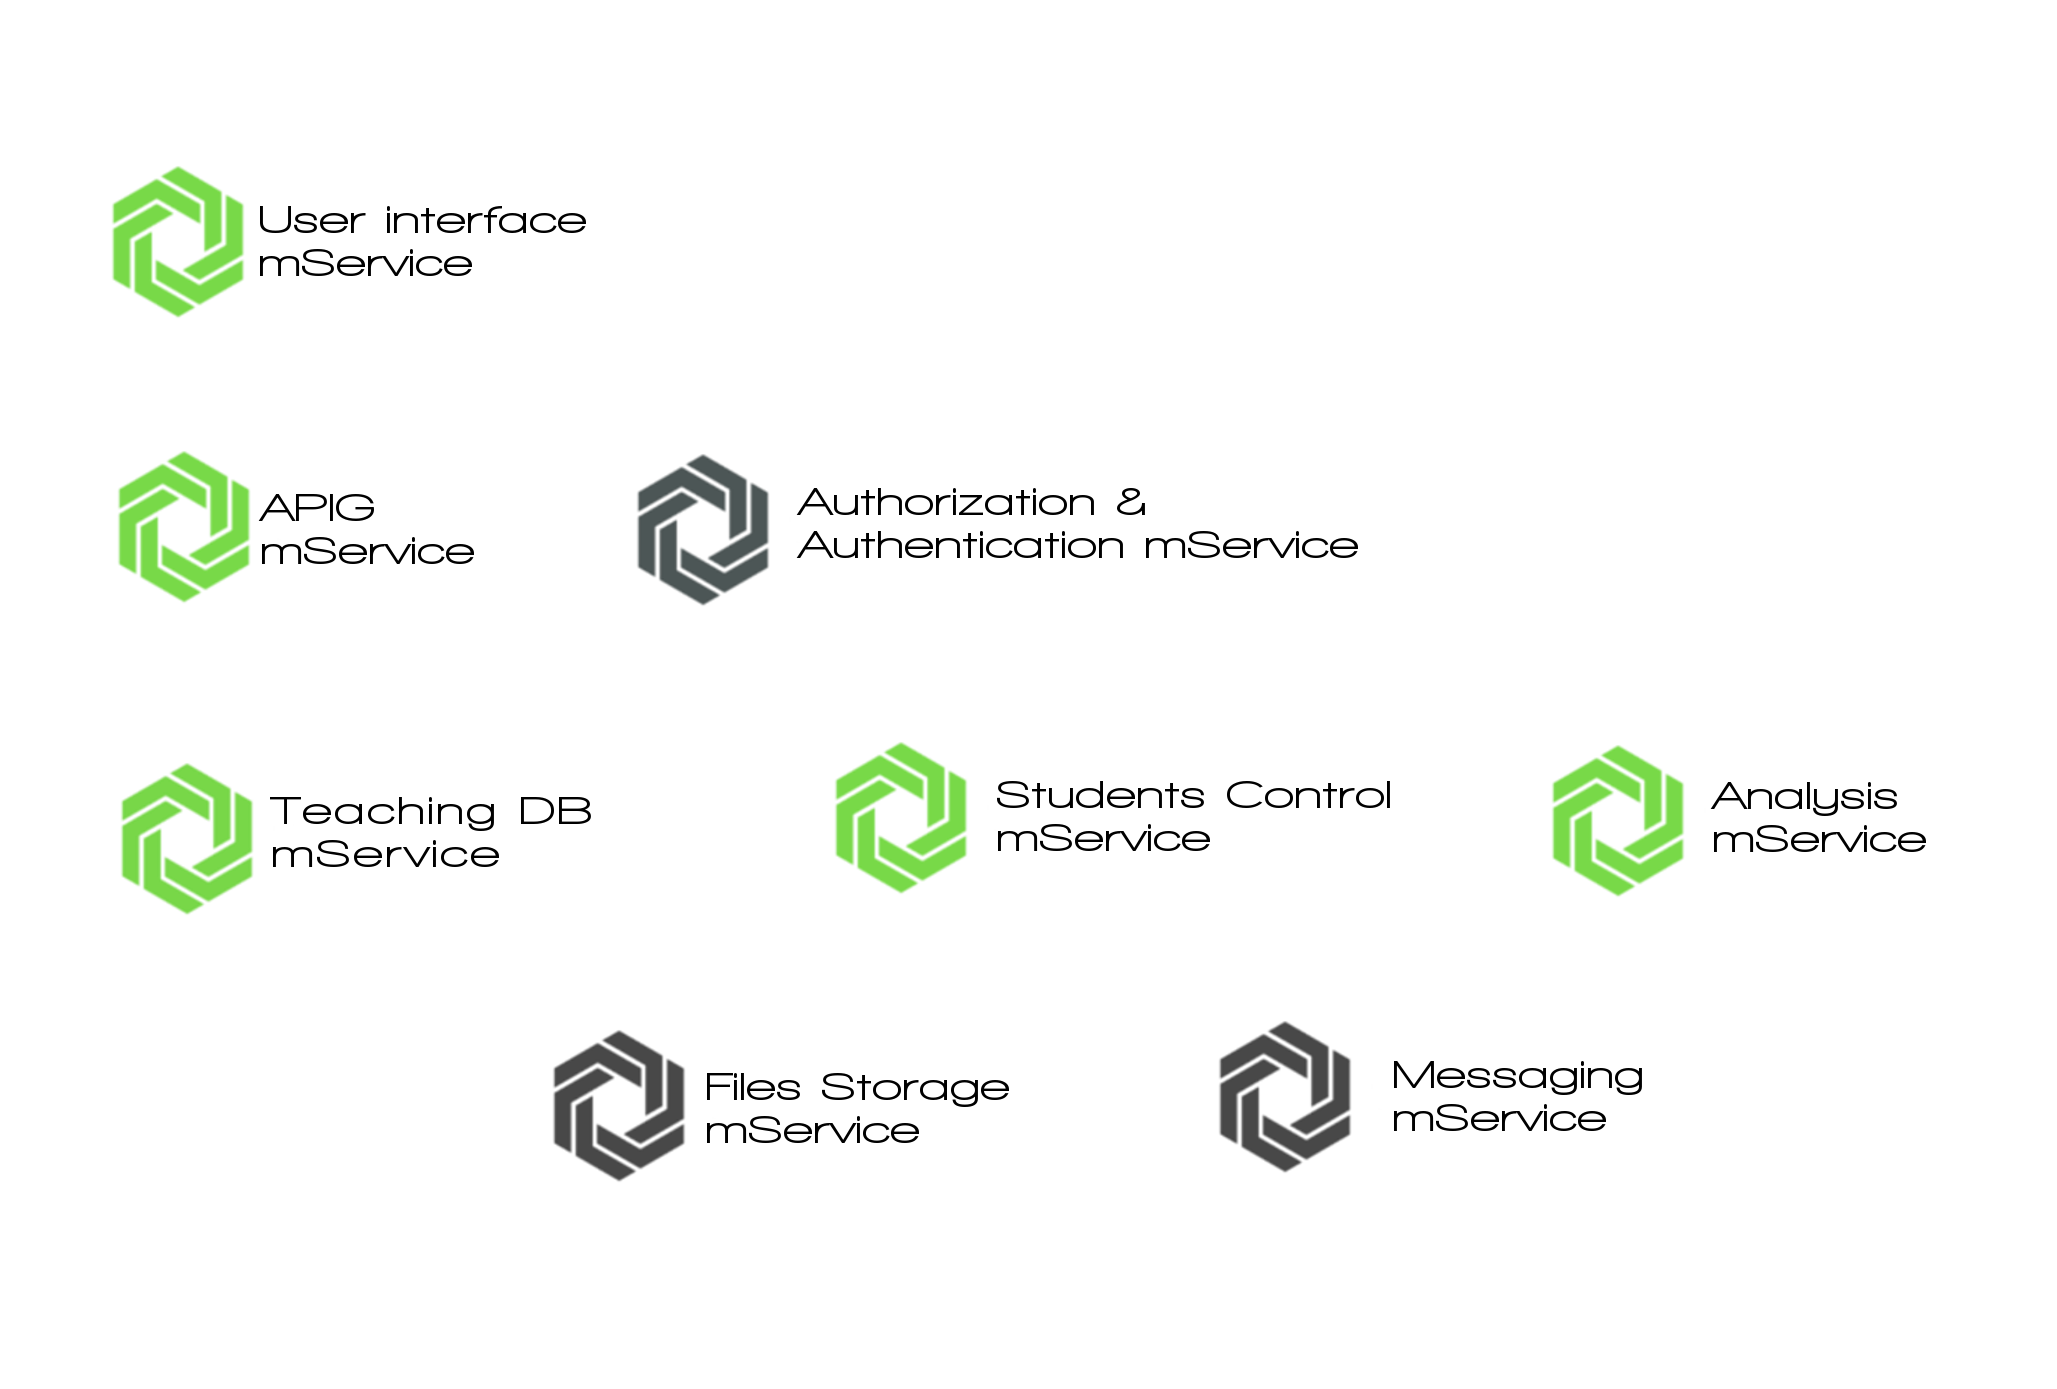
\includegraphics[scale=0.22]{img/graphics/final_microservices_distribution.png}
\end{center}

This is the real situation of the develop

\begin{center}
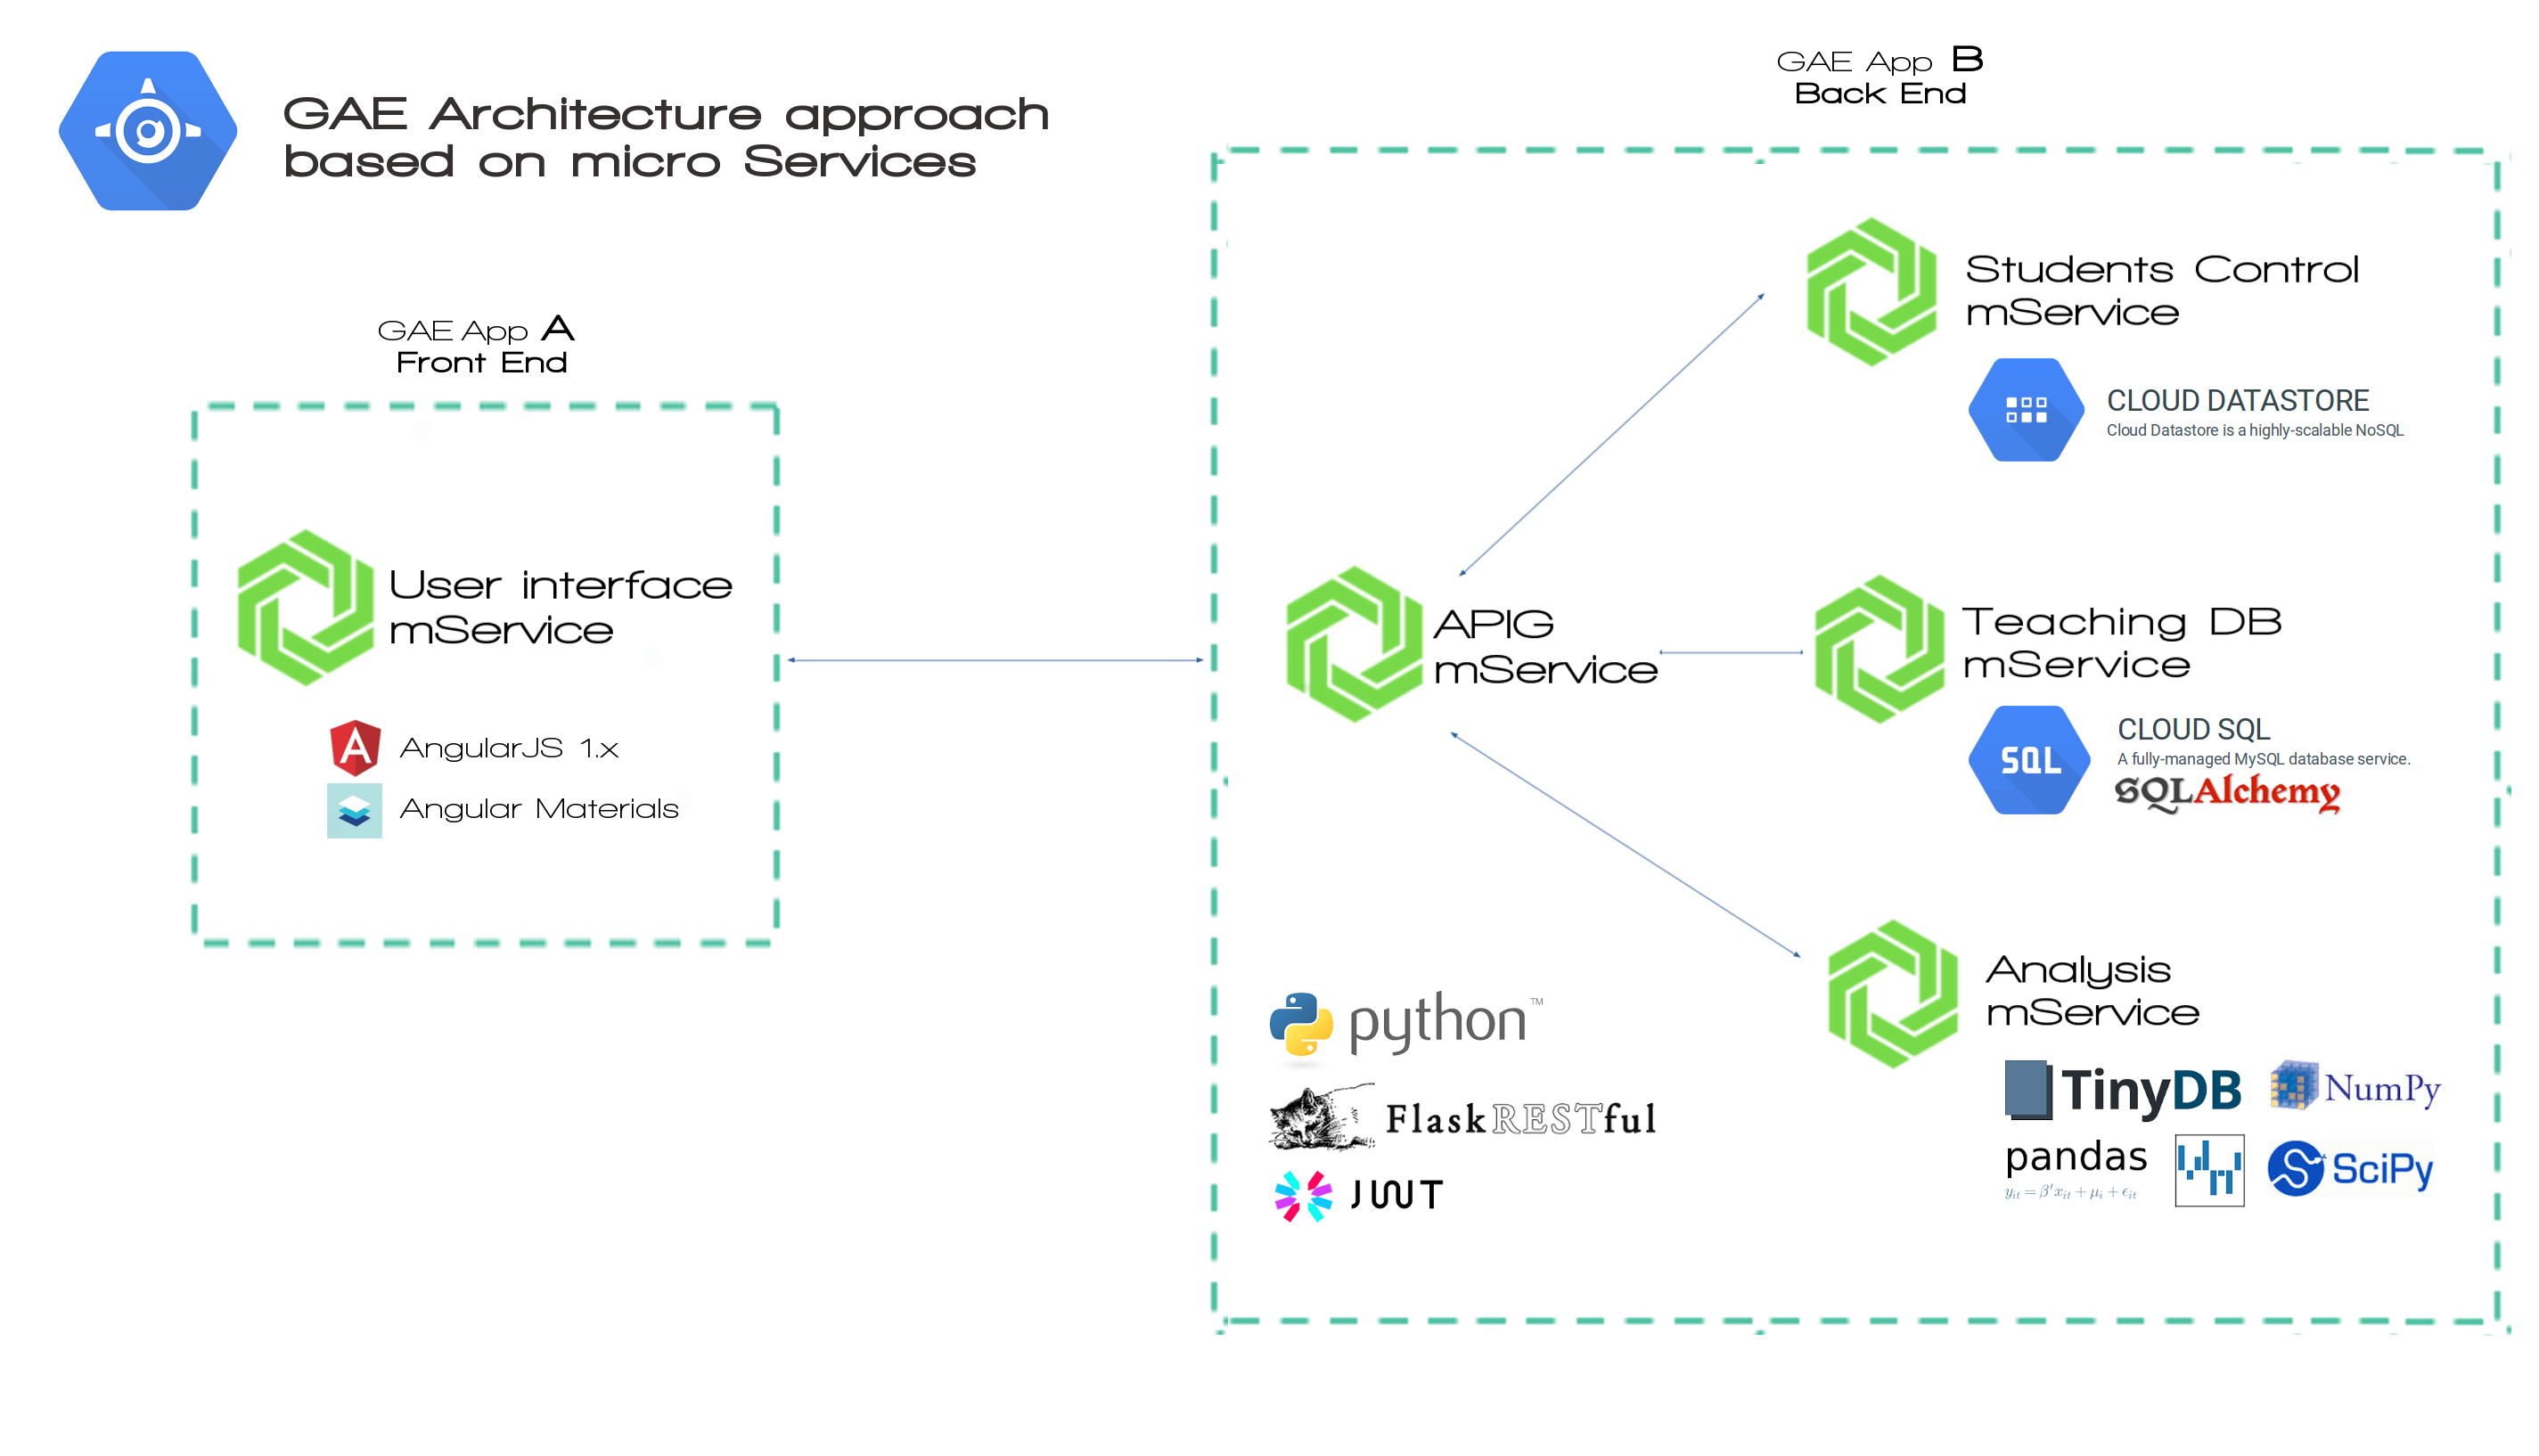
\includegraphics[scale=0.15]{img/graphics/GAE_final_architecture.png}
\end{center}

\subsection{API standar status code cases}

CODIGOS Y POR QUE ELEGIMOS LOS QUE ELEGIMOS

\subsection{API Gateway microService}

On the other had with docs something similar happens, don't have sense
write a doc defining the behaviour of all sections of api gateway
if this doc already exists in each service. It's redundant and complex
to mantain. Because of this a simple approach is link the docs to
services docs, so the task of write it relegate to them.

\subsubsection {API Definition}

\subsection{Teaching Data Base microService}


This mService offers the managment of the teaching of the center.
This means that persist in a relational database all relations between
teachers, students, subjects, etc, and all resource availables to
make this posible throuhg an api.\bigskip

This like the rest offers his resource throuhg an api writed in Flask
(follow the same architecture that all).

The engine to save all these relations is MySQL, for many reasons,
mainly because is the best known engine and in which it has some experience
and also because GCP offers as a cloud product Google Cloud SQL Databases.
Until recently only offerts MySQL but now (since March of 2017) they
offer also PostgreSQL.

\subsubsection{Design}


As base of requirements process have been used user stories.

\noindent\shadowbox{\begin{minipage}[t]{1\columnwidth - 2\fboxsep - 2\fboxrule - \shadowsize}%
\textbf{\#1 }

Me as manager, I want save subjects, teachers, students and classes.%
\end{minipage}}

\bigskip

\noindent\shadowbox{\begin{minipage}[t]{1\columnwidth - 2\fboxsep - 2\fboxrule - \shadowsize}%
\textbf{\#2}

Me as manager, I want can relate teachers with subjects.%
\end{minipage}}




\subsubsection{Access Library}

In the old version it was a little ORM that offers simple methods
to access data transform this in SQL raw sencentes. Now this library
is only a wraper of the SQLAlchemy to keep apart the apirest of the
service to the database access layer.

\begin{center}
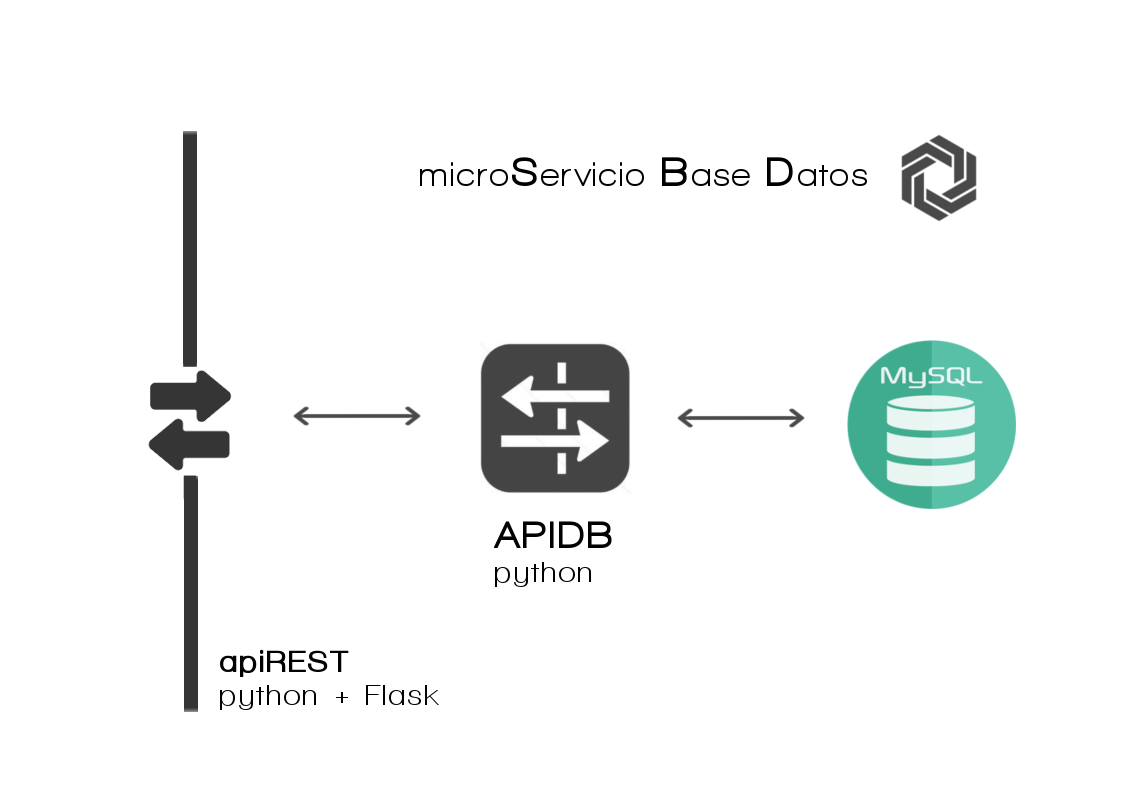
\includegraphics[scale=0.4]{img/graphics/dbms_diagram.png}
\end{center}

\subsubsection{Database logical design}

Based on user histories and the domain of the problem the designe
done based of this entity relation diagram:

The design follow some details that the domain presents, that is related
(at least the more significantly) below:

\begin{center}
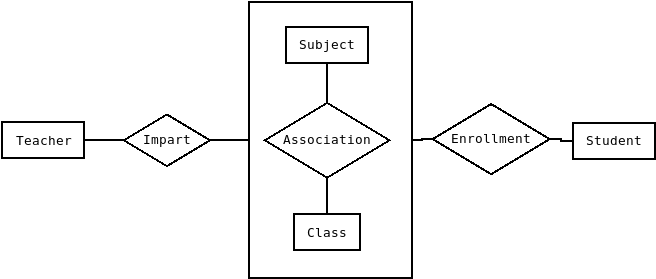
\includegraphics[scale=0.4]{img/diagrams/dbms-ER.png}
\end{center}



\subsubsection{Way to access to raw data}

While at firs of develop the mainly strategie to follow was write
all by cero, finally the point of view has been changed to follow
the use of standard tools and avoid reinvent the wheel.

So, if in the first stages of the project the acces to raw data through
the engine was hand made, using an own simple library that worked
like as simple ORM, the evolution of it and especially the problems
found and the unmaintainability of code have made that now the approach
turned to use a good tool as ORM like \href{http://www.google.es}{SQLAlchemy}.

The changes in the specifications of the api while the develop and
the maintaince of the performance of the queries when is writed hand
made in raw SQL isn't a good idea. Before the develop of this mService
it easy to understand that only in few projects is justified the use
of raw sql sencences and drivers whiout ORM (by easy that it was).


\subsection{Students Control microService}


\subsection{Analysis microService}
